% SPIN 2027 initial submission: anonymous, single column, no page numbers.
% Official Springer proceedings package: LLNCS v2.25, 03 September 2026.
% Compile with XeLaTeX and BibTeX (Overleaf runs the necessary passes).
\documentclass{llncs}
\usepackage[T1]{fontenc}
\usepackage{newtxtext}
\usepackage[varvw]{newtxmath}
\usepackage{graphicx}
\usepackage{booktabs,tabularx,array}
\usepackage{amsmath}
\usepackage{algorithm}
\usepackage{algpseudocode}
\usepackage{xurl}
\usepackage[hidelinks]{hyperref}
\urlstyle{same}
\emergencystretch=1em
\newcolumntype{Y}{>{\raggedright\arraybackslash}X}
\graphicspath{{figures/}}
\pagestyle{empty}
\begin{document}
\title{Memory-Pressure Forecasting and Growth-Based Warnings: An Empirical Study}
\author{}
\institute{}
\maketitle
\thispagestyle{empty}
\begin{abstract}
Forecasting rising memory pressure can support monitoring, but accurate forecasts do not by themselves identify memory leaks. We compare persistence, linear trend, restricted ARIMA and a small LSTM on one Antarex fault-injection recording and three Westermo industrial recordings, using chronological splits and 60- or 300-second horizons. Forecast error and growth-warning performance are evaluated separately. In the original Antarex run, LSTM reduces RMSE from ARIMA's 1.516 to 1.216 percentage points of RAM. Its warning rule, however, recognizes 34 of 35 injected events against trend-only's 35, with timestamp recall 0.466 versus 0.859. A matched study of five random seeds and two LSTM input configurations adds 40 runs. Extra features improve mean RMSE on only two of four recordings. Multivariate Antarex warning F1 is $0.571\pm0.031$, below trend-only's 0.830, and false alarm starts range from 43 to 137 against 86. Analyzing the saved scores shows that the original missed event occurred simply because the forecast-growth threshold was not reached. Because the Westermo dataset lacks verified leak ground truth, it can only support forecasting evaluations. Furthermore, while local replay and inference benchmarks confirm prototype viability, we have not yet validated live runtime performance or lead-time warnings prior to memory exhaustion.

\keywords{Memory pressure \and Time-series forecasting \and LSTM \and Warning evaluation \and Operating-system telemetry}
\end{abstract}

\section{Introduction}
An operating system can report growing memory use without identifying its cause. A larger workload, a cache, or an application retaining allocations can produce similar aggregate measurements. A forecast of memory availability is therefore a resource estimate, not proof of a memory leak. This distinction matters when a forecasting model is used to trigger operational warnings.

We study whether a more accurate short-horizon forecast gives more useful warnings on recorded telemetry. The target is the memory-pressure proxy
\begin{equation}
y_t=1-\frac{\operatorname{available\ memory}_t}{\operatorname{total\ physical\ memory}_t}.
\label{eq:target}
\end{equation}
It measures the fraction of RAM unavailable for immediate use. Models predict $y_{t+h}$ using observations through time $t$. Warning rules then assess recent growth, optionally requiring the forecast to indicate continued growth. These two tasks are evaluated separately.

The study uses controlled Antarex fault injections and three unlabeled Westermo industrial test-system recordings. Its contribution is empirical: (1) a reproducible comparison of forecast error and warning coverage under the same temporal evaluation protocol; (2) a matched five-seed comparison of memory-only and multivariate LSTMs; and (3) an explanation of a missed injected event using the saved decision scores. We also measure the local replay and inference prototype. We do not propose a new neural architecture, diagnose allocation-level causes, or demonstrate advance warning before memory exhaustion.

\section{Related Work and Research Gap}
Software-aging research links resource behavior, workload and failure. Measurement-based models estimate resource exhaustion~\cite{ref8}; web-server experiments examine aging under workload~\cite{ref9}. Surveys organize aging, rejuvenation and online failure-prediction methods~\cite{ref10,ref22}. These works establish the research direction; they do not imply that every rising RAM trace is a leak. Zhao et al. use injected leaks to study accelerated failures~\cite{ref11}, illustrating the additional outcome evidence needed to discuss exhaustion.

Different observation levels support different conclusions. Valgrind provides dynamic instrumentation~\cite{ref12}; adaptive profiling and methods using garbage-collector information inspect heap behavior~\cite{ref14,ref17}. Beneder et al. examine runtime measurements on embedded Linux~\cite{ref19}. Differential aging analysis compares software versions~\cite{ref20}. RESIN combines detection, diagnosis and mitigation in production infrastructure~\cite{ref21}. Our aggregate telemetry has neither heap-allocation traces nor paired software versions, so those diagnostic claims are outside its scope.

Jindal et al. detect leak patterns from memory-utilization histories using LBR and Precog variants~\cite{ref1}. Assi et al. compare Box--Jenkins and LSTM forecasts for Windows performance~\cite{ref2}. Statistical forecasting and simple benchmarks remain essential comparisons~\cite{ref24,ref25}. LSTM provides a learned sequence model~\cite{ref26}, but architecture studies and strong linear baselines caution against assuming that complexity ensures better forecasts~\cite{ref28,ref32}. Hybrid ARIMA--neural forecasting~\cite{ref29}, software-fault ARIMA--LSTM forecasting~\cite{ref30}, and hLSTM-Aging~\cite{ref31} use different model combinations. We evaluate separate predictors and do not reproduce their architectures or compare scores from different tasks.

Table~\ref{tab:related} summarizes the closest methodological contrasts. Its final column describes the boundary relevant to this study, rather than asserting that an earlier method is generally inadequate.
\begin{table}[htbp]
\caption{Selected earlier studies and the evidence they provide.}
\label{tab:related}
\small
\begin{tabularx}{\textwidth}{@{}p{2.15cm}YY@{}}
\toprule
Study & Observation and purpose & Boundary for the present comparison\\
\midrule
Jindal et al.~\cite{ref1} & Utilization histories; LBR/Precog leak-pattern methods & Their labels and algorithms differ from our injected-event and forecast-warning protocol.\\
Assi et al.~\cite{ref2} & Windows counters; ARIMA/LSTM forecast errors & Forecast-error ranking alone does not answer our timestamp/event warning question.\\
Zhao et al.~\cite{ref11} & Injected leaks; accelerated failure study & Failure outcomes are available there; our audited block has no exhaustion outcome.\\
Lou et al.~\cite{ref21} & Production service with detection, diagnosis and mitigation & Requires evidence beyond our aggregate replay and growth warnings.\\
Battisti et al.~\cite{ref31} & Hybrid neural model for software-aging forecasts & Different architecture and target setting; its scores cannot rank our warning rules.\\
Kim et al.~\cite{ref44} & Evaluation of time-series anomaly detection & Warns about point adjustment; we retain timestamp scores and separate event counts.\\
\bottomrule
\end{tabularx}
\end{table}

Assumptions and benchmark quality affect anomaly-detection results~\cite{ref40,ref45,ref46}. Forecast errors and warning scores assess different outcomes~\cite{ref41,ref42,ref43}. Chronological holdouts and training-only scaling make the information available at each prediction explicit~\cite{ref36,ref39}.

\noindent\textbf{Research gap.} On these recordings, it remains unclear whether lower forecast error improves growth-warning coverage, false-alarm frequency and recognition delay under one temporal protocol. We address this question using matched origins, injected-event labels, repeated seeds and a memory-only ablation. Unlabeled workload data support forecasting comparisons, not leak-detection claims.

\section{Data and Experimental Protocol}
Figure~\ref{fig:architecture} summarizes the archived workflow. The forecast and warning branches are evaluated separately: labels calibrate and score the warning rules, but never enter the predictors. The live sampler is a separate exploratory trend-only path, described in Algorithm~\ref{alg:pipeline}.

\begin{figure}[htbp]
\centering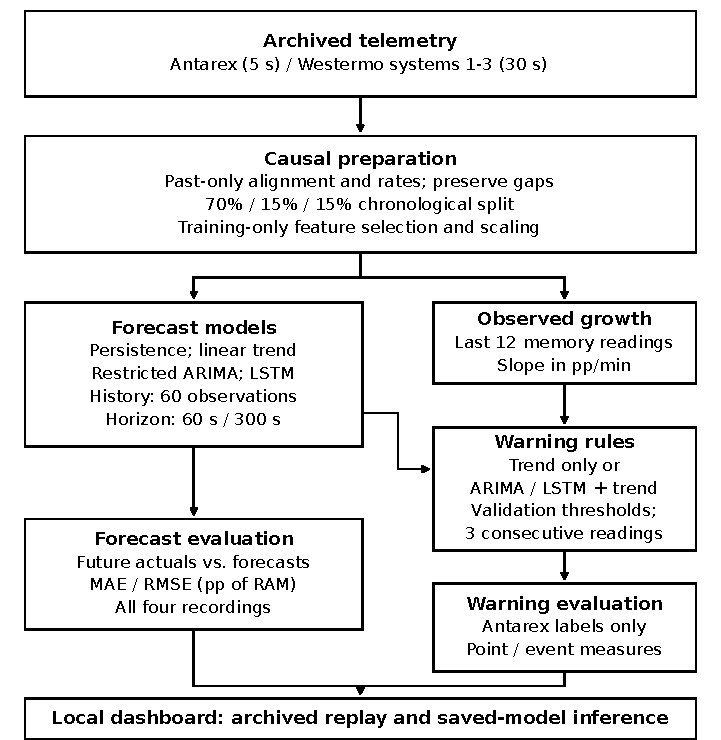
\includegraphics[width=\textwidth]{architecture.pdf}
\Description{Archived Antarex and Westermo telemetry undergo causal preparation and chronological splitting. Prepared observations feed forecasting models and a recent-memory-growth calculation. Forecasts are scored against future observations. Recent growth, optionally combined with ARIMA or LSTM forecast growth, produces warnings after three qualifying readings. Warning evaluation uses Antarex labels. The local dashboard displays archived replay and saved-model inference. Live sampling is a separate unvalidated path.}
\caption{Architecture of the archived experiment. Horizons are 60 s for Antarex and 300 s for Westermo. Only ARIMA and LSTM forecasts assist the growth rules; persistence and linear trend are forecast baselines. Warning evaluation separates timestamp precision, recall and F1 from event misses, false alarm starts and recognition delay. Westermo supports forecast scores and descriptive alarm counts, not labeled warning scores. The original ARIMA warning rule was disabled after validation. pp: percentage points of RAM.}
\label{fig:architecture}
\end{figure}

\subsection{Dataset Choice and Forecast Horizons}
Antarex was selected because it combines real machine telemetry with recorded and controlled fault injections~\cite{ref3,ref4,ref5}. The experiment uses the complete recovered CPU-MEM\_mono block, which covers approximately 12 days and contains 228 injected leak episodes. Only the metric streams required for this pipeline were included. The nested archive was verified using its recorded size and CRC. However, the complete outer archive was not acquired, and its published MD5 was not verified. Therefore, the dataset used in this study represents a defined subset rather than a validation of the entire Antarex release.

Westermo provides a complementary industrial workload consisting of 19 test systems monitored twice per minute over one month~\cite{ref6}. All 19 CSV files were acquired and checked against the repository metadata. For this pilot, systems 1--3 were selected in numerical order, with each system modeled separately. Since confirmed memory-leak labels are unavailable, these systems are used only for forecasting evaluation and descriptive alarm counts. Both datasets are available under CC BY 4.0, and their original attribution has been retained.

Antarex data is aligned to a five-second grid, whereas Westermo retains its native 30-second sampling interval. The preset forecasting horizons are 12 Antarex steps (60 s) and 10 Westermo steps (300 s). These settings allow both forecasts to look approximately ten observations ahead while accounting for the sampling interval of each dataset. They are practical settings for the pilot study and should not be considered validated optimal warning lead times. The same 60-observation history covers 295 s for Antarex and 1770 s for Westermo. As a result, error magnitudes across the two sources should not be treated as a controlled comparison over an equal physical time horizon.

\begin{table}[htbp]
\caption{Recording scope and eligible samples. A: Antarex; W1--W3: Westermo systems. Train is the eligible count before LSTM training stride.}
\label{tab:data}
\centering\small
\setlength{\tabcolsep}{5pt}
\begin{tabular}{@{}lrrrrr@{}}
\toprule
Recording & Grid rows & Train & Validation & Test & Inputs\\
\midrule
A &207361&145081&31032&31032&7\\
W1&86401&59691&12891&12891&8\\
W2&86401&60412&12891&12745&7\\
W3&86401&60412&12891&12891&8\\
\bottomrule
\end{tabular}
\end{table}

\subsection{Causal Preparation and Feature Availability}
For Antarex, the most recent source observation at or before each grid time is used, with a maximum age of 2.1 s. Differences between counter readings are used to calculate page-fault, swap, and disk rates based on the actual elapsed time. A rate is considered invalid if a counter resets, the time interval is nonpositive, or the interval exceeds 7.2 s. CPU features are calculated using non-overlapping tick categories. For Westermo, the published CPU and disk rates are used directly without further differentiation. Missing values and gaps are not interpolated.

The selected Antarex inputs include memory pressure, anonymous and committed memory, busy and I/O-wait CPU fractions, and total and major page-fault rates. Swap and monitored disk streams remain constant in the training partition and are therefore excluded. Westermo uses memory pressure, user/system/I/O-wait CPU rates, disk read/write rates, one-minute load, and swap use. For system 2, the constant swap input is removed. Westermo does not contain page-fault fields. Inputs with a training standard deviation of at most $10^{-12}$ are treated as constant. Their removal prevents undefined standardization and avoids adding uninformative inputs. However, this does not mean that disk or swap is unimportant for other workloads. The feature ablation described below evaluates the retained feature set as a whole rather than examining the causal effect of each individual feature.

Each recording is divided according to time into 70\% training, 15\% validation, and 15\% test sets. These boundaries are established before the windows are constructed. The training means and population standard deviations are then used to scale the subsequent data. A window is retained only if both its history and target fall within the same valid, contiguous segment and partition. The first Antarex row in each partition is excluded to prevent rate calculations from depending on observations from the preceding partition. Westermo systems 1 and 2 contain 652 and 8 missing grid rows, respectively. The memory-only ablation uses exactly the same coverage mask as the multivariate model, ensuring that differences in sample availability cannot explain the results.

For Antarex, the injection start and end times define half-open labeled intervals $[s,e)$. These intervals are checked against the supplied fault labels. IDs, timestamps, commands, and fault labels are not used as predictor inputs. The labels establish the controlled injection task, but no process-allocation measurements are available to confirm naturally occurring memory leaks. Additionally, a non-leak label may coincide with another injected fault, so it does not necessarily indicate that the system is healthy.

\subsection{Predictors and Repeated Runs}
Persistence repeats the latest memory pressure. Linear trend extends a least-squares line fitted to 12, 30 or 60 recent values; validation RMSE selects the window. Restricted ARIMA uses orders $(1,1,0)$, $(3,1,0)$ and $(5,1,0)$ without drift. Parameters are estimated by Yule--Walker on the longest contiguous training segment, and validation RMSE selects the order. This limited comparison does not implement a full Box--Jenkins search. Forecasts are clipped to $[0,1]$ for scoring.

Both LSTM variants use one unidirectional layer with 32 hidden units and a linear output from its final hidden state. The recurrent state resets for each window. Training uses standardized-target mean squared error, Adam at 0.001, batch size 64 and gradient clipping at 1.0. Training retains every twelfth eligible Antarex origin and every fourth Westermo origin; validation/test use all eligible origins. The best validation-RMSE checkpoint is selected from at most 20 epochs, with patience four. There is no dropout, bidirectional layer or hybrid ARIMA stage.

The original September Colab experiment used seed 42. The revision trains both feature variants from scratch with seeds 7, 21, 42, 84 and 123 on the same local CPU runtime: 40 runs in total. All checkpoints are frozen before the new test scores are computed. Every seed is reported, with mean and sample standard deviation (SD). This is variation from training randomness on fixed data, not uncertainty across new machines. Memory-only LSTM matches the baselines' input variable; model fitting and training sample use still differ. Fixed hidden width yields 4513 parameters for memory-only, versus 5281 or 5409 for seven or eight inputs. No new labeled recording is added.

\section{Warning Procedure and Evaluation}
\subsection{Growth Rules and Threshold Calibration}
Let $g_t$ be the least-squares slope over the latest 12 memory-pressure observations, expressed in percentage points (pp) of RAM per minute. For forecast $f_m(t)$ with horizon $h$ in seconds, define
\begin{equation}
q_m(t)=\frac{100[f_m(t)-y_t]}{h/60},\qquad
s_m(t)=\min\{g_t,q_m(t)\}.
\label{eq:score}
\end{equation}
Trend-only uses $s(t)=g_t$. Forecast-assisted warnings require both observed and forecast growth. A warning becomes active on the third consecutive eligible score at or above its threshold; one failure clears it. Gaps and split boundaries reset the count. Three readings suppress isolated excursions but add 10 s of confirmation at Antarex cadence and 60 s at Westermo cadence. This was a fixed engineering choice, not an optimized duration or a statistical-significance test. Mann--Kendall testing and autocorrelation corrections are alternative future comparisons~\cite{ref33,ref35}.

Each rule selects independently from $\{0.01,0.025,0.05,0.1,0.2,0.4,0.8,1.6,3.2\}$ pp/min and a disabled option. Antarex validation point F1 is maximized, with ties resolved by fewer false-positive timestamps and then the higher threshold; disabled ranks highest in the last tie-break. The original thresholds were 0.8 for trend-only and 0.4 for LSTM-assisted. Every ARIMA candidate produced zero validation warning timestamps after confirmation, so the disabled option won the tie. This describes the selected no-drift ARIMA and rule, not a general inability of ARIMA to support warnings. Each new LSTM run recalibrates on validation only; original results are preserved separately.

Algorithm~\ref{alg:pipeline} separates archived-model evaluation from the live monitor. The live branch records OS telemetry every five seconds using \texttt{psutil}, computes the same memory proxy and an exploratory observed-growth rule, and exports measurements. It does not apply the archived LSTM to incompatible Windows features.
\begin{algorithm}[t]
\caption{Telemetry forecasting and causal warning generation}
\label{alg:pipeline}
\begin{algorithmic}[1]
\Require Archived telemetry or live OS sampler; history 60; trend history 12
\If{archived experiment}
  \State Align past observations; derive rates; retain gaps and label provenance
  \State Split chronologically; fit scalers on training rows; form valid windows
  \State Fit predictors on training data; select checkpoints on validation RMSE
  \State Select warning thresholds using validation labels; freeze choices
\Else
  \State Initialize five-second sampler and exploratory trend threshold
\EndIf
\For{each new observation at time $t$}
  \State Read available telemetry; compute $y_t$ using Eq.~\ref{eq:target}
  \State Reset history/count after a gap; wait until history is sufficient
  \State Compute observed slope $g_t$ from the last 12 readings
  \If{compatible archived-model inputs}
    \State Scale history with saved training statistics; predict $f_m(t)$
    \State Set $s_t=g_t$ for trend-only or Eq.~\ref{eq:score} for assisted rules
  \Else
    \State Set $s_t=g_t$; do not substitute invented model inputs
  \EndIf
  \State Update consecutive qualifying count; warn when count $\geq3$
  \State Save forecast, score, warning and transition into alarm state
\EndFor
\State Score stored forecasts/decisions only where suitable outcomes exist
\end{algorithmic}
\end{algorithm}

\subsection{What Each Measure Means}
MAE is the average absolute difference between predicted and observed future pressure. RMSE squares the errors before averaging and taking the square root, giving large mistakes greater weight~\cite{ref41}. Both are reported in pp of total RAM. An RMSE of 1.5 pp describes forecast deviation on this scale; it is neither 98.5\% detection accuracy nor a bound on every error.

At each eligible origin, TP means a warning during a recorded leak, FP a warning outside one, and FN an active leak without a warning. Precision $=\mathrm{TP}/(\mathrm{TP+FP})$ asks how many warned timestamps are leak-active. Recall $=\mathrm{TP}/(\mathrm{TP+FN})$ asks how much labeled leak time is covered. F1 $=2\mathrm{TP}/(2\mathrm{TP+FP+FN})$ balances these two aspects. Zero-denominator ratios remain undefined. Imbalance makes these measures more informative than overall accuracy alone~\cite{ref42}.

An alarm start is an inactive-to-active transition, including activation after a gap. False alarm starts per non-leak hour (FA/h) divide starts outside injected-leak intervals by observed non-leak exposure: eligible non-leak origins times cadence. Persistent false warnings are also reported as false-positive minutes. These are distinct costs.

Event recognition requires a new alarm start inside a fully covered injected interval, with a covered sample immediately before it. A prior alarm does not count again. Event recall is recognized events divided by eligible events; detection delay is first alarm time minus injection start. Medians and 90th percentiles describe detected events only, so missed-event counts accompany them. Detecting one timestamp does not make every timestamp in that interval correct~\cite{ref43,ref44}. These delays measure recognition after injection begins, not warning lead time before exhaustion.

\section{Results and Interpretation}
\subsection{Forecast Accuracy and the Baseline Comparison}
Table~\ref{tab:original_forecast} preserves the original run. On Antarex, LSTM RMSE was 1.216 pp against ARIMA's 1.516 pp, a 19.8\% reduction, while MAE changed only from 0.363 to 0.358 pp. The larger RMSE improvement indicates a stronger effect on large errors than on average absolute error. Across Westermo, the original LSTM reduced RMSE but ARIMA had lower MAE: no method wins under every loss.

The selected Antarex ARIMA$(3,1,0)$ coefficients are approximately $-0.011$, $-0.010$ and $-0.011$. With no drift, forecast increments quickly become small, making its predictions close to persistence; their RMSEs differ by only 0.000196 pp. Linear extrapolation performs worse in all four recordings, consistent with transient slopes not continuing through the forecast horizon. Figure~\ref{fig:forecast} shows the fixed original example interval; full-test scores, rather than that interval, support the comparisons.


\begin{table}[htbp]
\caption{Original test forecast errors: MAE / RMSE, in percentage points (pp) of total RAM. A uses 60 s; W1--W3 use 300 s. LSTM is the single Colab seed-42 run.}
\label{tab:original_forecast}
\centering\small
\setlength{\tabcolsep}{4pt}
\begin{tabular}{@{}lrrrr@{}}
\toprule
Model & A & W1 & W2 & W3\\
\midrule
Persistence & 0.361 / 1.517 & 0.094 / 0.363 & 0.109 / 0.317 & 0.240 / 0.715\\
Linear trend & 0.377 / 1.744 & 0.145 / 0.376 & 0.144 / 0.348 & 0.329 / 0.818\\
ARIMA & 0.363 / 1.516 & 0.093 / 0.318 & 0.105 / 0.291 & 0.230 / 0.658\\
Original LSTM & 0.358 / 1.216 & 0.099 / 0.296 & 0.117 / 0.258 & 0.251 / 0.608\\
\bottomrule
\end{tabular}
\end{table}


\begin{figure}[htbp]
\centering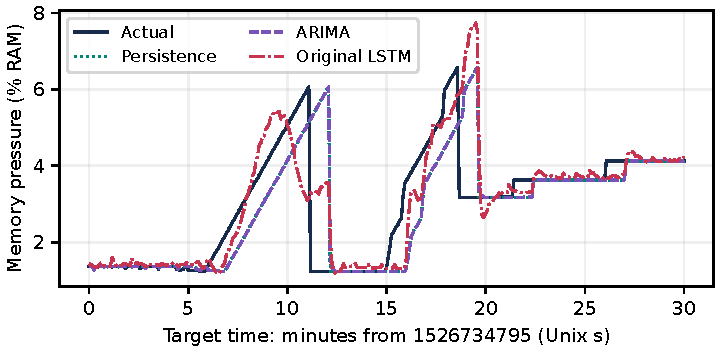
\includegraphics[width=\textwidth]{actual_predicted.pdf}
\Description{Actual and predicted memory pressure in percent of RAM over the fixed original first thirty minutes of Antarex test target times.}
\caption{Original Antarex 60-second-ahead rolling forecasts, aligned by target time. Predictions shown at a time were issued 60 s earlier. Persistence and ARIMA nearly overlap. This is the first fixed 30-minute test interval, not a best-case selection.}
\label{fig:forecast}
\end{figure}

\subsection{Random Seeds and the Memory-Only Ablation}
The new CPU runs use Python 3.12.14, PyTorch 2.8.0+cpu and two Torch threads. Table~\ref{tab:ablation} keeps them separate from Colab. On Antarex, multivariate mean RMSE is 1.204 pp versus memory-only 1.221 pp. Paired multivariate RMSE is lower in four of five Antarex seeds and all five W1 seeds, but only one W2 seed and no W3 seed. On W2 and W3, extra inputs also increase MAE in every paired seed. Additional telemetry therefore does not consistently improve this fixed model and training budget. The experiment does not isolate which feature helps or harms.

Both LSTM variants have lower mean RMSE than restricted ARIMA on each recording, but all their mean MAEs exceed ARIMA's. Training minimizes squared error, which weights large deviations strongly; lower RMSE with worse MAE is therefore possible. Seed SD describes optimization variability on these recordings, not a confidence interval for other systems. No additional labeled dataset or independent holdout was introduced.


\begin{table}[htbp]
\caption{Five-seed LSTM test errors: mean $\pm$ sample SD, in pp. Mem: memory-only; Multi: retained multivariate inputs. All five seeds are included.}
\label{tab:ablation}
\centering\small
\setlength{\tabcolsep}{4pt}
\begin{tabular}{@{}lrrrr@{}}
\toprule
Recording & MAE (Mem) & MAE (Multi) & RMSE (Mem) & RMSE (Multi)\\
\midrule
A & $0.378\pm0.018$ & $0.365\pm0.024$ & $1.221\pm0.015$ & $1.204\pm0.020$\\
W1 & $0.099\pm0.008$ & $0.103\pm0.008$ & $0.300\pm0.001$ & $0.297\pm0.002$\\
W2 & $0.110\pm0.005$ & $0.121\pm0.004$ & $0.260\pm0.003$ & $0.263\pm0.003$\\
W3 & $0.242\pm0.011$ & $0.278\pm0.026$ & $0.606\pm0.005$ & $0.618\pm0.009$\\
\bottomrule
\end{tabular}
\end{table}


\subsection{Warnings, Missed Events and Recognition Delay}
There are 1933 leak-active origins among 31,032 Antarex test origins and 35 fully covered injected events. Table~\ref{tab:original_warning} shows that the original LSTM warning improves precision and reduces false alarm starts from 86 to 42, but covers less leak-active time and misses one event. False alarm rates are 2.128/h for trend-only and 1.039/h for LSTM; false-positive exposure is 34.17 and 13.50 min respectively. Their detected-event 90th-percentile delays are 56.0 and 45.7 s. The disabled ARIMA rule is equivalent to always-off and misses all events.

The difference follows from the warning objective. Regression rewards accurate future levels over all origins, whereas the assisted rule demands both observed and forecast growth above a threshold for three readings. A model can predict the level closely while predicting insufficient continued growth. The additional condition suppresses some false alarms and some true warnings; minimizing forecast RMSE does not optimize event recall or warning F1.


\begin{table}[htbp]
\caption{Original Antarex test warnings. P/R: timestamp precision/recall; FA: false alarm starts; missed: events missed out of 35; delay: median seconds after injection among detected events only. A dash means undefined.}
\label{tab:original_warning}
\centering\small
\setlength{\tabcolsep}{4pt}
\begin{tabular}{@{}lrrrrrr@{}}
\toprule
Rule & P & R & F1 & FA & Missed & Delay (s)\\
\midrule
Trend only & 0.802 & 0.859 & 0.830 & 86 & 0 & 30\\
LSTM + trend & 0.848 & 0.466 & 0.601 & 42 & 1 & 31\\
ARIMA (off) & -- & 0.000 & 0.000 & 0 & 35 & --\\
\bottomrule
\end{tabular}
\end{table}


Event 1534, a low-intensity injection starting at 22:00:14 UTC on 19 May 2018, demonstrates this mechanism (Fig.~\ref{fig:missed}). During its 236 s and 47 eligible origins, forecast growth peaks at 0.216 pp/min, below the 0.4 threshold. Thus no reading can satisfy the forecast gate, irrespective of the three-reading requirement. Observed growth reaches 0.938 pp/min; trend-only warns after 56 s. Memory pressure spans approximately 3.20--7.17\%. The recorded scores explain the decision failure, not its allocation-level cause.

\begin{figure}[!htbp]
\centering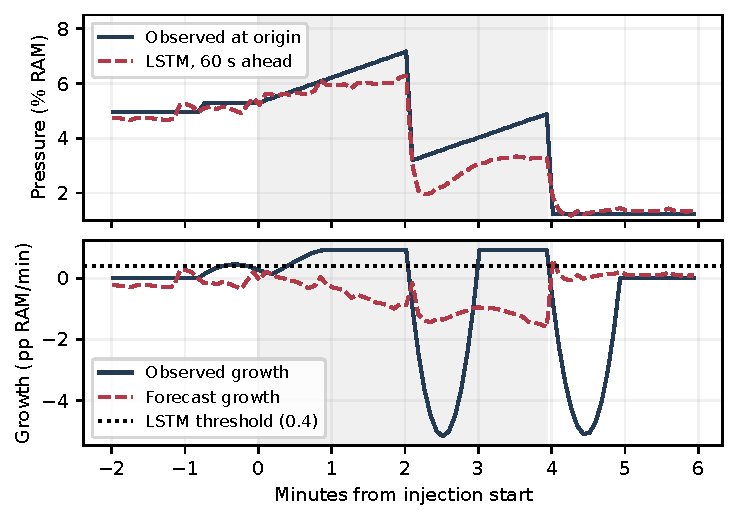
\includegraphics[width=\textwidth]{missed_event.pdf}
\Description{Two panels show memory pressure and growth scores around the original missed injection. Forecast growth stays below the warning threshold during the shaded interval.}
\caption{Original missed injected event 1534. Shading marks the recorded injection. Top: current pressure and the forecast issued at the same origin (its target is 60 s later). Bottom: observed and forecast growth; predicted growth remains below the LSTM gate throughout the injection. pp: percentage points of RAM.}
\label{fig:missed}
\end{figure}

The seed study weakens a general claim of fewer false alarms (Table~\ref{tab:repeat_warning}). Multivariate precision is $0.758\pm0.112$ and recall $0.461\pm0.010$; memory-only gives $0.648\pm0.071$ and $0.482\pm0.021$. Multivariate false starts range from 43 to 137, compared with the unchanged trend count of 86; memory-only ranges from 126 to 168. Each variant misses zero to two events depending on seed. Trend-only F1 remains 0.830, above every new LSTM-assisted run. The original precision/false-alarm advantage is therefore not stable across all repetitions. Validation selects thresholds separately for each run; forecast training variability and threshold decisions both influence these results.


\begin{table}[htbp]
\caption{Repeated LSTM-assisted Antarex warnings. F1 and FA/h are mean $\pm$ SD; missed is the range out of 35 events. Delay summarizes the five detected-event medians, not pooled events.}
\label{tab:repeat_warning}
\centering\small
\setlength{\tabcolsep}{4pt}
\begin{tabular}{@{}lrrrr@{}}
\toprule
Inputs & F1 & FA/h & Missed & Delay (s)\\
\midrule
Multivariate & $0.571\pm0.031$ & $2.014\pm1.052$ & 0--2 & $26.6\pm3.4$\\
Memory-only & $0.551\pm0.028$ & $3.405\pm0.449$ & 0--2 & $30.4\pm2.7$\\
\bottomrule
\end{tabular}
\end{table}


\subsection{Prototype Checks and Measurement Limits}
All 40 implementation tests passed, including loopback HTTP endpoints. Startup verified 76 source files covering 69,559 test origins. In a separate in-process benchmark on Windows with 8 logical CPUs and 7.8 GiB RAM, each recording received 100 replay/JSON requests and 100 warm model requests. Median replay times ranged from 7.05 to 21.84 ms; median warm inference ranged from 0.45 to 0.56 ms (95th percentiles 0.69--0.96 ms). All 404 first/warm inferences matched archived predictions within $10^{-6}$ pressure fraction. The first request, including library/model loading, took 5.34 s. Process resident memory increased from 25.4 to 402.3 MiB; this includes replay data, libraries and four models, not isolated monitoring overhead.

These measurements exclude HTTP transport and browser rendering. The live collector returned a Windows performance-counter error before any samples were recorded. No live timing, CPU-overhead or labeled live-detection result is reported. Longer live trials, missing-counter resilience and controlled overhead measurements remain unvalidated. The optional live mode uses exploratory trend warnings, not the archived Linux LSTM.


\section{Limitations, Reproducibility and Conclusion}
The expanded study still uses one labeled Antarex recording, controlled injections, overlapping windows and reused holdouts. Earlier test forecasts were inspected during development before the original warning protocol was finalized. Five-seed repetition measures optimization variability; it does not remove that development dependence. The multivariate/memory-only comparison controls history, origins and training settings but changes input dimension and parameter count. It cannot attribute improvement to an individual feature. Selected horizons, thresholds and confirmation length also require independent validation.

Antarex never reaches the illustrative 80\% pressure level in the audited block; its peak is approximately 42.24\%. No exhaustion or crash outcome is observed. The study therefore makes no claim of warning before memory runs out. Such a claim needs labeled trials with resource limits, observed depletion times and warning lead times, including failures to warn. Westermo cannot establish real-leak detection because its leak labels are unknown. Additional labeled recordings, process-level allocation evidence, matched multivariate statistical baselines, independent temporal holdouts and longer compatible live trials remain future work.

\paragraph{Reproducibility.} The project retains preprocessing, baseline, LSTM and warning code, four executable notebooks, model configurations, weights, origin indices, checksums and scoring scripts. The revision adds a fixed seed/feature protocol, per-run forecasts and warning outcomes, a missed-event analysis and a prototype benchmark. Reproduction uses the verified input package, runs the seed study, then independently checks saved predictions and warning scores. The repository is currently private; these materials are not claimed to be publicly accessible. A masked supplementary code package accompanies this revision for author review, while raw/derived data packages require separate access. Public dataset sources are cited above; a public code release or reviewer-access route must be arranged before claiming open reproducibility.

\begin{samepage}
\paragraph{Conclusion.} Lower forecasting error and better warning performance are different outcomes. LSTM reduced RMSE compared to restricted ARIMA, but trend-only covered more labeled time and had higher warning F1. The original LSTM precision/false-alarm benefit was not consistent across seeds. Additional features improved mean RMSE on only two of four recordings, and the missed-event scores exposed a failed forecast-growth gate. These findings assist in evaluating forecast accuracy and operational warnings separately. They do not establish production leak diagnosis or pre-exhaustion warning; independent labeled trials, process measurements and longer live evaluation are the next tests.
\end{samepage}

\begin{credits}
\subsubsection*{Disclosure of Interests.} The authors have no competing interests relevant to this study.
\end{credits}

\bibliographystyle{splncs04}
\bibliography{references}
\end{document}
